
\section{Introduction}

Improving the efficiency of computation has always been one of the prime goals of computing.
Program performance can be improved significantly by reaping the benefits of parallelism, temporal and spatial locality, and other performance sources. Relevant program transformations are particularly tedious and challenging when targeting modern multicore CPUs and GPUs with deep memory hierarchies and parallelism, and are often performed automatically by optimizing compilers.

The polyhedral model enables precise analyses and a relatively easy specification of transformations (loop restructuring, automatic parallelization, etc.) that take advantage of hardware performance sources.  As a result, there is growing evidence that the polyhedral model is one of the best frameworks for efficient transformation of compute-intensive programs~\cite{tc,teckyl,mullapudi2015polymage},
% \az{I rephrased "machine learning programs" because we don't target ML programs specifically}
% agreed -wm
and for programming accelerator architectures~\cite{cerebras_chip,ppcg,tc_cim}. Consequently, the compiler community has focused on building tools that identify and optimize parts of the program that can be represented within the polyhedral model (commonly referred to as static-control parts, or \scop's). Such tools tend to\rz{Maybe just say there are two categories? And could we explicitly say one uses lower-level repr. and the other is rather higher-level (just to connect with the final paragraphs)?} fall into two categories.

% \az{I rewrote the two paragraphs below significantly. We are not contributing better \scop detection... (I understand there has been some work to implement that, but this is not exactly novel, sorry about that). Neither do we use hardware-specific things like vectorization.}
% \wmnote{agreed, I do wonder if there's anything more we can add as potential downsides of source style as its a bit bare}
% \az{We can, but we will not be using that later, so it can be used against us :)}
% fair point -wm, some good future work for sure :P

Compiler-based tools like Polly~\cite{grosser.ppl.2012} and Graphite~\cite{pop2006graphite} detect and transform {\scop}s in compiler intermediate representations (IRs). While this offers seamless integration with rest of the compiler, the lack of high-level structure and information hinders the tools' ability to perform analyses and transformations. This structure needs to be recovered from optimized IR, often imperfectly or at a significant cost~\cite{delinearization}. Moreover, common compiler optimizations such as LICM may interfere with the process~\cite{delicm}. Finally, low-level IRs often lack constructs for, e.g., parallelism or reductions, produced by the transformation, which makes the flow more complex.

\begin{figure}
\begin{center}
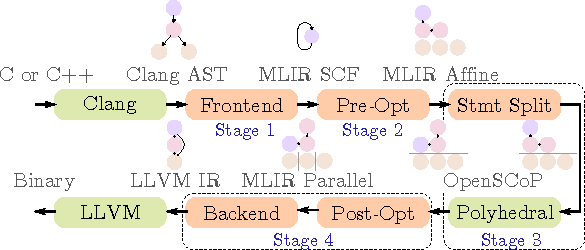
\includegraphics[scale=0.7]{images/mixed.pdf}
\caption{The \tool compilation flow consists of 4 stages. The frontend traverses Clang AST to emit MLIR SCF dialect (Section~\ref{sec:frontsub}), which is raised to the Affine dialect and pre-optimized (Section~\ref{sec:raising}). The IR is then processed by a polyhedral scheduler (Sections~\ref{sec:polyhedral_tools},\ref{sec:stmt_splitting}) before post-optimization and parallelization (Section~\ref{sec:opts}). Finally, it is translated to LLVM IR for further optimization and binary generation by LLVM.}
\label{fig:pipeline}
\end{center}
\end{figure}

Source-to-source compilers such as Pluto~\cite{Bondhugula2008Pluto}, \textsc{PoCC}~\cite{pocc} and \textsc{ppcg}~\cite{ppcg} operate directly on C or C++ code. While this can effectively leverage the high-level information from source code, the effectiveness of such tools is often reduced by the lack of enabling optimizations such as those converting hazardous memory loads into single-assignment virtual registers. Furthermore, the transformation results must be expressed in C, which is known to be complex~\cite{cloog,grosser2015polyhedral} and is also missing constructs for, e.g., reduction loops or register values not backed by memory storage.


This paper proposes and evaluates the benefits of a polyhedral compilation flow, \tool (Figure~\ref{fig:pipeline}), that can leverage both the high-level structure available in source code and the fine-grained control of compiler optimization provided by low-level IRs. It builds on the recent MLIR compiler infrastructure that allows the interplay of multiple abstraction levels within the same representation, during the same transformations~\cite{mlir}. Intermixable MLIR abstractions, or \emph{dialects}, include high-level constructs such as loops, parallel and reduction patterns; low-level representations fully covering LLVM IR~\cite{llvm}; and a polyhedral-inspired representation featuring loops and memory accesses annotated with affine expressions.
%However, there are presently no polyhedral scheduling transformations within MLIR.
% \rz{I feel that this line is a bit detached with the rest. Could we say things like ``Polygeist is the 1st tool that includes polyhedral scheduling transformations'' after this line.}
% \az{\tool is BY FAR not the first tool that includes polyhedral scheduling. I think we are better off without this claim.}
% \wmnote{basically was thinking of a way to say that mlir currently didn't schedule (to prevent the argument of oh you just used an existing thing, though perhaps thats not an actual concern), is this reasonable to say now or stil should be axed}
% \az{There \emph{are} polyhedral transformations in mlir, just no affine scheduling, and we are using some of those, i.e. parallelization. I wrote it... Uday has a preprint on optimizing matmul to BLIS level with MLIR. We are shooting ourselves by saying this.}
% \wmnote{Yeah I'm now convinced there's no good way to concisely describe what we want to say from this (i.e. a potential problem that is solved by creating polymer) without losing attention in all the details}
Moreover, by combining the best of source-level and IR-level tools in an end-to-end polyhedral flow, \tool preserves high-level information and leverages them to perform new or improved optimizations, such as statement splitting and loop-carried value detection, on a \emph{lower}-level abstraction as well as to influence downstream optimizations.

We make the following contributions:
\begin{itemize}
    \item a C and C++ frontend for MLIR that preserves high-level loop structure from the original source code;
    \item an end-to-end flow with raising to and lowering from the polyhedral model, leveraging our abstraction to perform more optimizations than both source- and IR-level tools, including reduction parallelization;
    \item an exploration of new transformation opportunities created by \tool, in particular, statement splitting;
    \item and an end-to-end comparison between \tool and state-of-the-art source- and IR-based tools (Pluto~\cite{Bondhugula2008Pluto} and Polly~\cite{grosser2015polyhedral}) along with optimization case studies.
\end{itemize}
%\az{Had to kill the result preview for space reasons}
%\tool achieves the largest speedups when evaluated on the Polybench suite~\cite{polybench} both serially and in parallel. 